% !TEX TS-program = pdfLaTeX+shellescape
% !TEX encoding = UTF-8 Unicode

\documentclass[class=beamer,tikz]{standalone}
\setbeamertemplate{navigation symbols}{} % For delete the navigation symbols
\usepackage{pgfplots}
\pgfplotsset{compat=1.17}
\usetikzlibrary{angles}

\begin{document}
    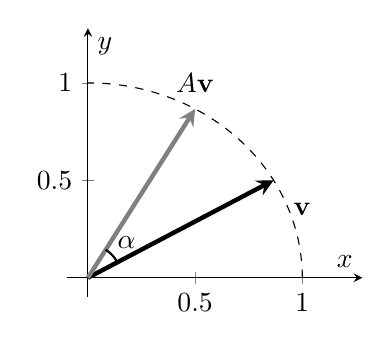
\begin{tikzpicture}[baseline]
        \begin{axis}[
            scale=0.6,xmin=-0.1,xmax=1.28,ymin=-0.1,ymax=1.28,
            legend style={at={(axis cs: 1,0)}, anchor=south east},
            unit vector ratio = {1,1},
            axis lines = middle,
            xlabel = {$x$}, ylabel = {$y$}, % axis labels
        ]
            \coordinate (A) at (axis cs:0,0);
            \coordinate (B) at (axis cs:0.866,0.5);
            \coordinate (C) at (axis cs:0.5,0.866);
            \draw[ultra thick,->,>=stealth] (A) -- (B);
            \draw[ultra thick,->,>=stealth,color=gray] (A) -- (C);
            \node at (axis cs: 1,0.35) {$\mathbf{v}$};
            \node at (axis cs: 0.5,1.0) {$A\mathbf{v}$};
            \addplot[samples=100,domain=0:90,dashed]({cos(x)},{sin(x)});
            \draw pic[draw,thick,angle eccentricity=1.5,angle radius=12]{angle=B--A--C};
            \node at (axis cs: 0.18,0.18) {$\alpha$};
        \end{axis}
    \end{tikzpicture}
\end{document}